\chapter*{ПРИЛОЖЕНИЯ}
\addcontentsline{toc}{chapter}{ПРИЛОЖЕНИЯ}

\section*{Приложение А. Блок-схемы алгоритмов}
\addcontentsline{toc}{section}{Приложение А. Блок-схемы алгоритмов}

\renewcommand{\thefigure}{А.\arabic{figure}}
\setcounter{figure}{0}
\begin{figure}[H]
\centering
\begin{tikzpicture}[
    node distance=1.5cm,
    every node/.style={font=\footnotesize},
    startstop/.style={draw, rectangle, rounded corners=10pt, minimum width=3.2cm,
      minimum height=0.8cm, align=center, fill=white},
    process/.style={draw, rectangle, minimum width=3.2cm, minimum height=0.9cm,
      align=center, fill=white},
    io/.style={draw, trapezium, trapezium left angle=75, trapezium right angle=105,
      trapezium stretches=true, minimum width=3.5cm, minimum height=0.8cm,
      align=center, fill=white},
    decision/.style={draw, diamond, aspect=2.5, minimum width=3cm,
      minimum height=0.8cm, align=center, fill=white},
    arrow/.style={thick,->,>=stealth}
]
\node (start)  [startstop] {Начало};
\node (pro1)   [process,  below of=start] {Суммирование PTS, FGA, FTA};
\node (pro2)   [process,  below of=pro1]
  {$D = 2 \cdot (\mathrm{FGA} + 0{,}44 \cdot \mathrm{FTA})$};
\node (dec1)   [decision, below of=pro2, yshift=-0.5cm] {$D = 0$?};
\node (pro3a)  [io,  right of=dec1, xshift=3.5cm] {Вывод:\\ значение не определено};
\node (pro3b)  [io,  below of=dec1, yshift=-0.5cm]
  {Возврат $\mathrm{PTS} / D$};
\node (stop)   [startstop, below of=pro3b] {Конец};

\draw [arrow] (start)  -- (pro1);
\draw [arrow] (pro1)   -- (pro2);
\draw [arrow] (pro2)   -- (dec1);
\draw [arrow] (dec1)   -- node[anchor=south] {Да}  (pro3a);
\draw [arrow] (dec1)   -- node[anchor=east]  {Нет} (pro3b);
\draw [arrow] (pro3b)  -- (stop);
\draw [arrow] (pro3a)  |- (stop);
\end{tikzpicture}
\caption{Схема алгоритма вычисления функции \texttt{calculate\_ts}}
\label{fig:algo-ts}
\end{figure}

\begin{figure}[H]
\centering
\begin{tikzpicture}[
    node distance=1.8cm,
    every node/.style={font=\footnotesize},
    startstop/.style={draw, rectangle, rounded corners=10pt,
      minimum width=4.5cm, minimum height=0.8cm,
      align=center, fill=white},
    process/.style={draw, rectangle,
      minimum width=4.5cm, minimum height=0.8cm,
      align=center, fill=white},
    io/.style={draw, trapezium, trapezium left angle=75, trapezium right angle=105,
      trapezium stretches=true, minimum width=4.5cm, minimum height=0.8cm,
      align=center, fill=white},
    decision/.style={draw, diamond, aspect=3,
      minimum width=4.5cm, minimum height=0.8cm,
      align=center, fill=white},
    arrow/.style={thick,->,>=stealth}
]
\node (start)  [startstop] {Начало};
\node (agg)    [process,  below of=start] {Суммирование FGM, FG3M, FGA из \\ \texttt{game\_player\_stats}};
\node (dec1)   [decision, below of=agg] {$\mathrm{FGA} = 0$?};
\node (null1)  [io,  right of=dec1, xshift=4.5cm] {Вывод:\\ значение не определено};
\node (ret)    [io,  below of=dec1] {Возврат $\displaystyle\frac{\mathrm{FGM}+0{,}5\cdot\mathrm{FG3M}}{\mathrm{FGA}}$};
\node (stop)   [startstop, below of=ret] {Конец};

\draw [arrow] (start) -- (agg);
\draw [arrow] (agg)   -- (dec1);
\draw [arrow] (dec1)  -- node[above] {Да} (null1);
\draw [arrow] (dec1)  -- node[right] {Нет} (ret);
\draw [arrow] (ret)   -- (stop);
\draw [arrow] (null1.east) -- ++(0.6,0) |- (stop);
\end{tikzpicture}
\caption{Схема алгоритма вычисления функции \texttt{calculate\_efg}}
\label{fig:algo-efg}
\end{figure}

\begin{figure}[H]
\centering
\begin{tikzpicture}[
    node distance=1.8cm,
    every node/.style={font=\footnotesize},
    startstop/.style={draw, rectangle, rounded corners=10pt,
      minimum width=4.5cm, minimum height=0.8cm,
      align=center, fill=white},
    process/.style={draw, rectangle,
      minimum width=4.5cm, minimum height=0.8cm,
      align=center, fill=white},
    io/.style={draw, trapezium, trapezium left angle=75, trapezium right angle=105,
      trapezium stretches=true, minimum width=4.5cm, minimum height=0.8cm,
      align=center, fill=white},
    decision/.style={draw, diamond, aspect=3,
      minimum width=4.5cm, minimum height=0.8cm,
      align=center, fill=white},
    arrow/.style={thick,->,>=stealth}
]
\node (start)  [startstop] {Начало};
\node (tid)    [process,  below of=start] {Определить team\_id \\ (параметр или последняя игра)};
\node (dec0)   [decision, below of=tid, yshift=-0.2cm] {team\_id IS NULL?};
\node (null0)  [io,  right of=dec0, xshift=4.5cm] {Вывод:\\ значение не определено};
\node (aggP)   [process,  below of=dec0, yshift=-0.2cm] {Суммирование FGA, FTA, \\ TOV, MP игрока};
\node (dec1)   [decision, below of=aggP, yshift=-0.2cm] {$\mathrm{MP} < 1$?};
\node (null1)  [io,  right of=dec1, xshift=4.5cm] {Вывод:\\ значение не определено};
\node (aggT)   [process,  below of=dec1, yshift=-0.2cm] {Суммирование TmFGA, TmFTA, \\ TmTOV, TmMP команды в общих матчах};
\node (dec2)   [decision, below of=aggT, yshift=-0.2cm] {denom $= 0$?};
\node (null2)  [io,  right of=dec2, xshift=4.5cm] {Вывод:\\ значение не определено};
\node (ret)    [io,  below of=dec2, yshift=-0.2cm] {Возврат $\displaystyle\frac{(\mathrm{FGA}+0{,}44\cdot\mathrm{FTA}+\mathrm{TOV})\cdot\frac{\mathrm{TmMP}}{5}}{\mathrm{MP}\cdot(\mathrm{TmFGA}+0{,}44\cdot\mathrm{TmFTA}+\mathrm{TmTOV})}$};
\node (stop)   [startstop, below of=ret] {Конец};

\draw [arrow] (start) -- (tid);
\draw [arrow] (tid)   -- (dec0);
\draw [arrow] (dec0)  -- node[above] {Да} (null0);
\draw [arrow] (dec0)  -- node[right] {Нет} (aggP);
\draw [arrow] (aggP)  -- (dec1);
\draw [arrow] (dec1)  -- node[above] {Да} (null1);
\draw [arrow] (dec1)  -- node[right] {Нет} (aggT);
\draw [arrow] (aggT)  -- (dec2);
\draw [arrow] (dec2)  -- node[above] {Да} (null2);
\draw [arrow] (dec2)  -- node[right] {Нет} (ret);
\draw [arrow] (ret)   -- (stop);

\draw [arrow] (null0.east) -- ++(0.5,0) coordinate (bus) |- (stop);
\draw [arrow] (null1.east) -- (null1.east -| bus);
\draw [arrow] (null2.east) -- (null2.east -| bus);
\end{tikzpicture}
\caption{Схема алгоритма вычисления функции \texttt{calculate\_usg}}
\label{fig:algo-usg}
\end{figure}

\begin{figure}[H]
\centering
\begin{tikzpicture}[
    node distance=1.8cm,
    every node/.style={font=\footnotesize},
    startstop/.style={draw, rectangle, rounded corners=10pt,
      minimum width=5.6cm, minimum height=0.8cm,
      align=center, fill=white},
    process/.style={draw, rectangle,
      minimum width=5.6cm, minimum height=0.8cm,
      align=center, fill=white},
    io/.style={draw, trapezium, trapezium left angle=75, trapezium right angle=105,
      trapezium stretches=true, minimum width=5.6cm, minimum height=0.8cm,
      align=center, fill=white},
    decision/.style={draw, diamond, aspect=3.4,
      minimum width=5.6cm, minimum height=0.8cm,
      align=center, fill=white},
    arrow/.style={thick,->,>=stealth}
]
\node (start) [startstop] {Начало};
\node (agg)   [process,  below of=start] {Суммирование PTS, TRB, AST, STL, BLK, \\ TOV, PF, FGM/FGA, FTM/FTA, MP};
\node (dec1)  [decision, below of=agg] {$\mathrm{MP} < 50$?};
\node (null1) [io,  right of=dec1, xshift=5cm] {Вывод:\\ значение не определено};
\node (uper)  [process,  below of=dec1] {$\mathrm{uPER} = (\mathrm{PTS}+\mathrm{TRB}+\ldots - \mathrm{TOV}-\mathrm{PF}-\Delta\mathrm{FG}-0{,}44\cdot\Delta\mathrm{FT}) \cdot \tfrac{48}{\mathrm{MP}}$};
\node (lg)    [process,  below of=uper] {Вычисление lg\_aPER: \\ AVG(uPER) по игрокам с MP $> 100$};
\node (dec2)  [decision, below of=lg] {lg\_aPER $= 0$ или NULL?};
\node (fix)   [process,  right of=dec2, xshift=5cm] {lg\_aPER $= 15{,}0$};
\node (ret)   [io,  below of=dec2] {Возврат $\mathrm{uPER} \cdot 15\,/\,\mathrm{lg\_aPER}$};
\node (stop)  [startstop, below of=ret] {Конец};

\draw [arrow] (start) -- (agg);
\draw [arrow] (agg)   -- (dec1);
\draw [arrow] (dec1)  -- node[above] {Да} (null1);
\draw [arrow] (dec1)  -- node[right] {Нет} (uper);
\draw [arrow] (uper)  -- (lg);
\draw [arrow] (lg)    -- (dec2);
\draw [arrow] (dec2)  -- node[above] {Да} (fix);
\draw [arrow] (dec2)  -- node[right] {Нет} (ret);
\draw [arrow] (fix)   |- (ret);
\draw [arrow] (ret)   -- (stop);
\draw [arrow] (null1.east) -- ++(1.0,0) |- (stop);
\end{tikzpicture}
\caption{Схема алгоритма вычисления функции \texttt{calculate\_per}}
\label{fig:algo-per}
\end{figure}

\begin{figure}[H]
\centering
\begin{tikzpicture}[
    node distance=1.8cm,
    every node/.style={font=\footnotesize},
    startstop/.style={draw, rectangle, rounded corners=10pt,
      minimum width=5.6cm, minimum height=0.8cm,
      align=center, fill=white},
    process/.style={draw, rectangle,
      minimum width=5.6cm, minimum height=0.8cm,
      align=center, fill=white},
    io/.style={draw, trapezium, trapezium left angle=75, trapezium right angle=105,
      trapezium stretches=true, minimum width=5.6cm, minimum height=0.8cm,
      align=center, fill=white},
    decision/.style={draw, diamond, aspect=3.4,
      minimum width=5.6cm, minimum height=0.8cm,
      align=center, fill=white},
    arrow/.style={thick,->,>=stealth}
]
\node (start) [startstop] {Начало};
\node (agg)   [process,  below of=start] {Суммирование PTS, TRB, AST, STL, \\ BLK, TOV, PF, MP из \texttt{game\_player\_stats}};
\node (dec1)  [decision, below of=agg] {$\mathrm{MP} < 50$?};
\node (null1) [io,  right of=dec1, xshift=5cm] {Вывод:\\ значение не определено};
\node (norm)  [process,  below of=dec1] {Нормировка на 100 мин: $X_{100} = X \cdot 100\,/\,\mathrm{MP}$};
\node (raw)   [process,  below of=norm, text width=6cm] {raw $= 0{,}123\cdot\mathrm{PTS}_{100}+0{,}234\cdot\mathrm{TRB}_{100}+0{,}689\cdot\mathrm{AST}_{100}$ \\ $+\,0{,}445\cdot\mathrm{STL}_{100}+0{,}407\cdot\mathrm{BLK}_{100}-0{,}605\cdot\mathrm{TOV}_{100}-0{,}086\cdot\mathrm{PF}_{100}$};
\node (lg)    [process,  below of=raw] {Вычисление lg\_avg: \\ AVG(raw) по игрокам с MP $> 100$};
\node (ret)   [io,  below of=lg] {Возврат raw $-$ lg\_avg};
\node (stop)  [startstop, below of=ret] {Конец};

\draw [arrow] (start) -- (agg);
\draw [arrow] (agg)   -- (dec1);
\draw [arrow] (dec1)  -- node[above] {Да} (null1);
\draw [arrow] (dec1)  -- node[right] {Нет} (norm);
\draw [arrow] (norm)  -- (raw);
\draw [arrow] (raw)   -- (lg);
\draw [arrow] (lg)    -- (ret);
\draw [arrow] (ret)   -- (stop);
\draw [arrow] (null1.east) -- ++(0.6,0) |- (stop);
\end{tikzpicture}
\caption{Схема алгоритма вычисления функции \texttt{calculate\_bpm}}
\label{fig:algo-bpm}
\end{figure}

\begin{figure}[H]
\centering
\begin{tikzpicture}[
    node distance=1.8cm,
    every node/.style={font=\footnotesize},
    startstop/.style={draw, rectangle, rounded corners=10pt,
      minimum width=5.6cm, minimum height=0.8cm,
      align=center, fill=white},
    process/.style={draw, rectangle,
      minimum width=5.6cm, minimum height=0.8cm,
      align=center, fill=white},
    io/.style={draw, trapezium, trapezium left angle=75, trapezium right angle=105,
      trapezium stretches=true, minimum width=5.6cm, minimum height=0.8cm,
      align=center, fill=white},
    decision/.style={draw, diamond, aspect=3.4,
      minimum width=5.6cm, minimum height=0.8cm,
      align=center, fill=white},
    arrow/.style={thick,->,>=stealth}
]
\node (start) [startstop] {Начало};
\node (get)   [io,  below of=start] {Получить status, home/away\_id, \\ счёт из \texttt{games} по game\_id};
\node (dec1)  [decision, below of=get] {status $\neq$ 'Finished' \\ или счёт NULL?};
\node (skip)  [io,  right of=dec1, xshift=5cm] {Возврат NEW/OLD};
\node (loop)  [process,  below of=dec1] {Для каждой команды в матче: SUM(points)};
\node (dec2)  [decision, below of=loop] {SUM $\neq$ ожидаемый счёт?};
\node (exc)   [io,  right of=dec2, xshift=5cm] {RAISE EXCEPTION};
\node (ret)   [io,  below of=dec2] {Возврат NEW/OLD};
\node (stop)  [startstop, below of=ret] {Конец};

\draw [arrow] (start) -- (get);
\draw [arrow] (get)   -- (dec1);
\draw [arrow] (dec1)  -- node[above] {Да} (skip);
\draw [arrow] (dec1)  -- node[right] {Нет} (loop);
\draw [arrow] (loop)  -- (dec2);
\draw [arrow] (dec2)  -- node[above] {Да} (exc);
\draw [arrow] (dec2)  -- node[right] {Нет} (ret);
\draw [arrow] (ret)   -- (stop);

\draw [arrow] (skip.east) -- ++(0.6,0) coordinate (bus) |- (stop);
\draw [arrow] (exc.east) -- (exc.east -| bus);
\end{tikzpicture}
\caption{Схема алгоритма функции-триггера \texttt{trg\_validate\_team\_score\_row}}
\label{fig:algo-trg-score}
\end{figure}

\begin{figure}[H]
\centering
\begin{tikzpicture}[
    node distance=1.8cm,
    every node/.style={font=\footnotesize},
    startstop/.style={draw, rectangle, rounded corners=10pt,
      minimum width=5.2cm, minimum height=0.8cm,
      align=center, fill=white},
    process/.style={draw, rectangle,
      minimum width=5.2cm, minimum height=0.8cm,
      align=center, fill=white},
    io/.style={draw, trapezium, trapezium left angle=75, trapezium right angle=105,
      trapezium stretches=true, minimum width=5.2cm, minimum height=0.8cm,
      align=center, fill=white},
    decision/.style={draw, diamond, aspect=3.2,
      minimum width=5.2cm, minimum height=0.8cm,
      align=center, fill=white},
    arrow/.style={thick,->,>=stealth}
]
\node (start) [startstop] {Начало};
\node (get)   [io,  below of=start] {Получить season\_id из \texttt{games} \\ по MAX(game\_id) вставленных строк};
\node (dec1)  [decision, below of=get] {season\_id IS NULL?};
\node (null1) [io,  right of=dec1, xshift=4.5cm] {Вывод:\\ значение не определено};
\node (call)  [process,  below of=dec1] {\texttt{CALL update\_season\_stats(season\_id)}};
\node (ret)   [io,  below of=call] {Вывод:\\ значение не определено};
\node (stop)  [startstop, below of=ret] {Конец};

\draw [arrow] (start) -- (get);
\draw [arrow] (get)   -- (dec1);
\draw [arrow] (dec1)  -- node[above] {Да} (null1);
\draw [arrow] (dec1)  -- node[right] {Нет} (call);
\draw [arrow] (call)  -- (ret);
\draw [arrow] (ret)   -- (stop);
\draw [arrow] (null1.east) -- ++(0.6,0) |- (stop);
\end{tikzpicture}
\caption{Схема алгоритма функции-триггера \texttt{trigger\_update\_season\_stats}}
\label{fig:algo-trg-update}
\end{figure}

\begin{figure}[H]
\centering
\begin{tikzpicture}[
    node distance=1.1cm,
    every node/.style={font=\footnotesize},
    startstop/.style={draw, rectangle, rounded corners=10pt, minimum width=5.2cm,
      minimum height=0.75cm, text centered, fill=white},
    process/.style={draw, rectangle, minimum width=5.2cm, minimum height=0.75cm,
      text centered, fill=white},
    arrow/.style={thick,->,>=stealth}
]
\node (start) [startstop] {Начало транзакции};
\node (pro1)  [process, below of=start]
  {GROUP BY player\_id, team\_id: базовые агрегаты};
\node (pro2)  [process, below of=pro1]
  {Подзапрос TmFGA/TmFTA/TmTOV по (game\_id, team\_id) для USG};
\node (pro3)  [process, below of=pro2]
  {Двухпроходный расчёт лигового среднего (PER, BPM)};
\node (pro4)  [process, below of=pro3]
  {Вызов calculate\_efg, ts, usg, per, bpm};
\node (pro5)  [process, below of=pro4]
  {UPSERT в player\_season\_stats};
\node (stop)  [startstop, below of=pro5] {Конец транзакции};

\draw [arrow] (start) -- (pro1);
\draw [arrow] (pro1)  -- (pro2);
\draw [arrow] (pro2)  -- (pro3);
\draw [arrow] (pro3)  -- (pro4);
\draw [arrow] (pro4)  -- (pro5);
\draw [arrow] (pro5)  -- (stop);
\end{tikzpicture}
\caption{Схема алгоритма хранимой процедуры \texttt{update\_season\_stats}}
\label{fig:algo-update}
\end{figure}

\section*{Приложение Б. Скрипты создания структуры базы данных}
\addcontentsline{toc}{section}{Приложение Б. Скрипты создания структуры базы данных}

\begin{lstlisting}[language=SQL]
CREATE TABLE positions (
    position_id SERIAL PRIMARY KEY,
    code VARCHAR(2) UNIQUE NOT NULL,
    name VARCHAR(20) NOT NULL
);

CREATE TABLE seasons (
    season_id SERIAL PRIMARY KEY,
    label VARCHAR(9) UNIQUE NOT NULL,
    start_date DATE NOT NULL,
    end_date DATE NOT NULL,
    season_type VARCHAR(15) NOT NULL
);

CREATE TABLE teams (
    team_id SERIAL PRIMARY KEY,
    nba_team_id INT UNIQUE NOT NULL,
    name VARCHAR(60) UNIQUE NOT NULL,
    abbreviation CHAR(3) UNIQUE NOT NULL,
    city VARCHAR(50) NOT NULL,
    conference VARCHAR(4) NOT NULL,
    arena_name VARCHAR(80),
    founded_year SMALLINT,
    is_active BOOLEAN DEFAULT TRUE
);
\end{lstlisting}

\section*{Приложение В. Примеры SQL-запросов}
\addcontentsline{toc}{section}{Приложение В. Примеры SQL-запросов}

\renewcommand{\thelstlisting}{В.\arabic{lstlisting}}
\setcounter{lstlisting}{0}
\begin{lstlisting}[language=SQL, label=lst:sql-filter,
  caption=Фильтрация игроков по позиции]
SELECT player_id, first_name, last_name
FROM players
WHERE position_id = (SELECT position_id FROM positions WHERE code = 'C')
  AND is_active = TRUE
ORDER BY last_name
LIMIT 10;
\end{lstlisting}
\begin{lstlisting}[language=SQL, label=lst:sql-join,
  caption=Результаты матчей с JOIN по сезону и командам]
SELECT
    s.label        AS season,
    g.game_date,
    ht.name        AS home_team,
    g.home_score,
    g.away_score,
    at.name        AS away_team,
    g.overtime
FROM games g
JOIN seasons s  ON s.season_id  = g.season_id
JOIN teams  ht  ON ht.team_id   = g.home_team_id
JOIN teams  at  ON at.team_id   = g.away_team_id
WHERE s.label = '2023-24'
  AND g.status = 'Finished'
ORDER BY g.game_date
LIMIT 10;
\end{lstlisting}
\begin{lstlisting}[language=SQL, label=lst:sql-group,
  caption=Агрегация сезонной статистики по позициям]
SELECT
    p.code                          AS position,
    COUNT(DISTINCT pss.player_id)   AS player_count,
    ROUND(AVG(pss.avg_pts), 2)      AS avg_pts,
    ROUND(AVG(pss.avg_reb), 2)      AS avg_reb,
    ROUND(AVG(pss.avg_ast), 2)      AS avg_ast,
    ROUND(AVG(pss.per),     2)      AS avg_per
FROM player_season_stats pss
JOIN players   pl ON pl.player_id   = pss.player_id
JOIN positions p  ON p.position_id  = pl.position_id
JOIN seasons   s  ON s.season_id    = pss.season_id
WHERE s.label = '2023-24'
  AND pss.avg_min >= 15
GROUP BY p.code
ORDER BY avg_per DESC;
\end{lstlisting}
\begin{lstlisting}[language=SQL, label=lst:sql-subquery,
  caption=Сравнение PER игрока со средним по лиге]
SELECT
    pl.first_name || ' ' || pl.last_name AS player,
    t.abbreviation                        AS team,
    pss.per,
    pss.avg_pts
FROM player_season_stats pss
JOIN players pl ON pl.player_id = pss.player_id
JOIN teams   t  ON t.team_id    = pss.team_id
WHERE pss.season_id = (SELECT season_id FROM seasons WHERE label = '2023-24')
  AND pss.per > (
      SELECT AVG(per)
      FROM player_season_stats
      WHERE season_id = (SELECT season_id FROM seasons WHERE label = '2023-24')
        AND per IS NOT NULL
  )
ORDER BY pss.per DESC
LIMIT 10;
\end{lstlisting}
\begin{lstlisting}[language=SQL, label=lst:sql-union,
  caption=Объединение топ-5 по очкам и передачам]
(SELECT 'Scoring'           AS category,
        pl.first_name || ' ' || pl.last_name AS player,
        pss.avg_pts         AS value
 FROM player_season_stats pss
 JOIN players pl ON pl.player_id = pss.player_id
 WHERE pss.season_id = (SELECT season_id FROM seasons WHERE label = '2023-24')
 ORDER BY pss.avg_pts DESC
 LIMIT 5)

UNION ALL

(SELECT 'Assists',
        pl.first_name || ' ' || pl.last_name,
        pss.avg_ast
 FROM player_season_stats pss
 JOIN players pl ON pl.player_id = pss.player_id
 WHERE pss.season_id = (SELECT season_id FROM seasons WHERE label = '2023-24')
 ORDER BY pss.avg_ast DESC
 LIMIT 5);
\end{lstlisting}


\section*{Приложение Г. Скрипты создания функций и процедур}
\addcontentsline{toc}{section}{Приложение Г. Скрипты создания функций и процедур}

\renewcommand{\thelstlisting}{Г.\arabic{lstlisting}}
\setcounter{lstlisting}{0}

\begin{lstlisting}[language=SQL]
CREATE OR REPLACE FUNCTION calculate_efg(
    p_player_id INT,
    p_season_id INT,
    p_team_id   INT DEFAULT NULL
)
RETURNS DECIMAL(5,4)
LANGUAGE plpgsql
STABLE
AS $$
DECLARE
    v_fgm NUMERIC := 0;
    v_fg3m NUMERIC := 0;
    v_fga NUMERIC := 0;
BEGIN
    SELECT
        COALESCE(SUM(gps.fgm), 0),
        COALESCE(SUM(gps.fg3m), 0),
        COALESCE(SUM(gps.fga), 0)
    INTO v_fgm, v_fg3m, v_fga
    FROM game_player_stats gps
    JOIN games g ON g.game_id = gps.game_id
    WHERE gps.player_id = p_player_id
      AND g.season_id   = p_season_id
      AND (p_team_id IS NULL OR gps.team_id = p_team_id);

    IF v_fga = 0 THEN
        RETURN NULL;
    END IF;

    RETURN ROUND((v_fgm + 0.5 * v_fg3m) / v_fga, 4);
END;
$$;
\end{lstlisting}

\begin{lstlisting}[language=SQL, label=lst:ts,
  caption=Реализация функции \texttt{calculate\_ts} (фрагмент)]
CREATE OR REPLACE FUNCTION calculate_ts(
    p_player_id INT, p_season_id INT, p_team_id INT DEFAULT NULL
) RETURNS DECIMAL(5,4) LANGUAGE plpgsql STABLE AS $$
DECLARE
    v_pts NUMERIC; v_fga NUMERIC; v_fta NUMERIC; v_denom NUMERIC;
BEGIN
    SELECT COALESCE(SUM(gps.points), 0),
           COALESCE(SUM(gps.fga), 0),
           COALESCE(SUM(gps.fta), 0)
    INTO v_pts, v_fga, v_fta
    FROM game_player_stats gps
    JOIN games g ON g.game_id = gps.game_id
    WHERE gps.player_id = p_player_id
      AND g.season_id = p_season_id
      AND (p_team_id IS NULL OR gps.team_id = p_team_id);

    IF v_fga = 0 AND v_fta = 0 THEN RETURN NULL; END IF;

    v_denom := 2.0 * (v_fga + 0.44 * v_fta);
    IF v_denom = 0 THEN RETURN NULL; END IF;

    RETURN ROUND(v_pts::DECIMAL / v_denom, 4);
END; $$;
\end{lstlisting}

\begin{lstlisting}[language=SQL, label=lst:trigger,
  caption=Триггер проверки корректности очков (фрагмент)]
CREATE OR REPLACE FUNCTION trg_validate_team_score_row()
RETURNS TRIGGER LANGUAGE plpgsql AS $$
DECLARE
    v_sum INT; v_expected INT;
BEGIN
    IF v_expected IS NOT NULL AND v_sum <> v_expected THEN
        RAISE EXCEPTION
            'Player points sum (%) does not match team score (%)',
            v_sum, v_expected;
    END IF;
    RETURN COALESCE(NEW, OLD);
END; $$;
\end{lstlisting}

\begin{lstlisting}[language=SQL, label=lst:grants,
  caption=Разграничение доступа командами привилегий]
GRANT SELECT ON ALL TABLES IN SCHEMA public TO analyst;
GRANT EXECUTE ON ALL FUNCTIONS IN SCHEMA public TO analyst;

GRANT SELECT ON v_team_stats   TO reader;
GRANT SELECT ON v_top_players  TO reader;
\end{lstlisting}

\section*{Приложение Д. Исходный код механизма кэширования}
\addcontentsline{toc}{section}{Приложение Д. Исходный код механизма кэширования}

В приложении приведён обобщённый декоратор с ключом по пути и строке запроса.
В реализованных маршрутах API (листинг~\ref{lst:cache-aside-pattern},
технологический раздел) применяется явный формат ключа
\texttt{leaders:\{metric\}:\{season\_id\}:...}, что обеспечивает точечную
инвалидацию по шаблонам при вызове \texttt{POST /admin/refresh}.

\begin{lstlisting}[language=Python]
import json
from functools import wraps
from fastapi import Request, Response

def cache_response(ttl_seconds: int = 300):
    def decorator(func):
        @wraps(func)
        async def wrapper(*args, **kwargs):
            request: Request = kwargs.get("request")
            redis_client = request.app.state.redis
            
            cache_key = f"api_cache:{request.url.path}?{request.url.query}"
            
            cached_data = await redis_client.get(cache_key)
            if cached_data:
                return Response(
                    content=cached_data, 
                    media_type="application/json"
                )
                
            response = await func(*args, **kwargs)
            
            await redis_client.setex(
                cache_key, 
                ttl_seconds, 
                json.dumps(response)
            )
            return response
        return wrapper
    return decorator
\end{lstlisting}

\section*{Приложение Е. Пользовательский интерфейс программного комплекса}
\addcontentsline{toc}{section}{Приложение Е. Пользовательский интерфейс программного комплекса}

\renewcommand{\thefigure}{Е.\arabic{figure}}
\setcounter{figure}{0}

\begin{figure}[H]
\centering
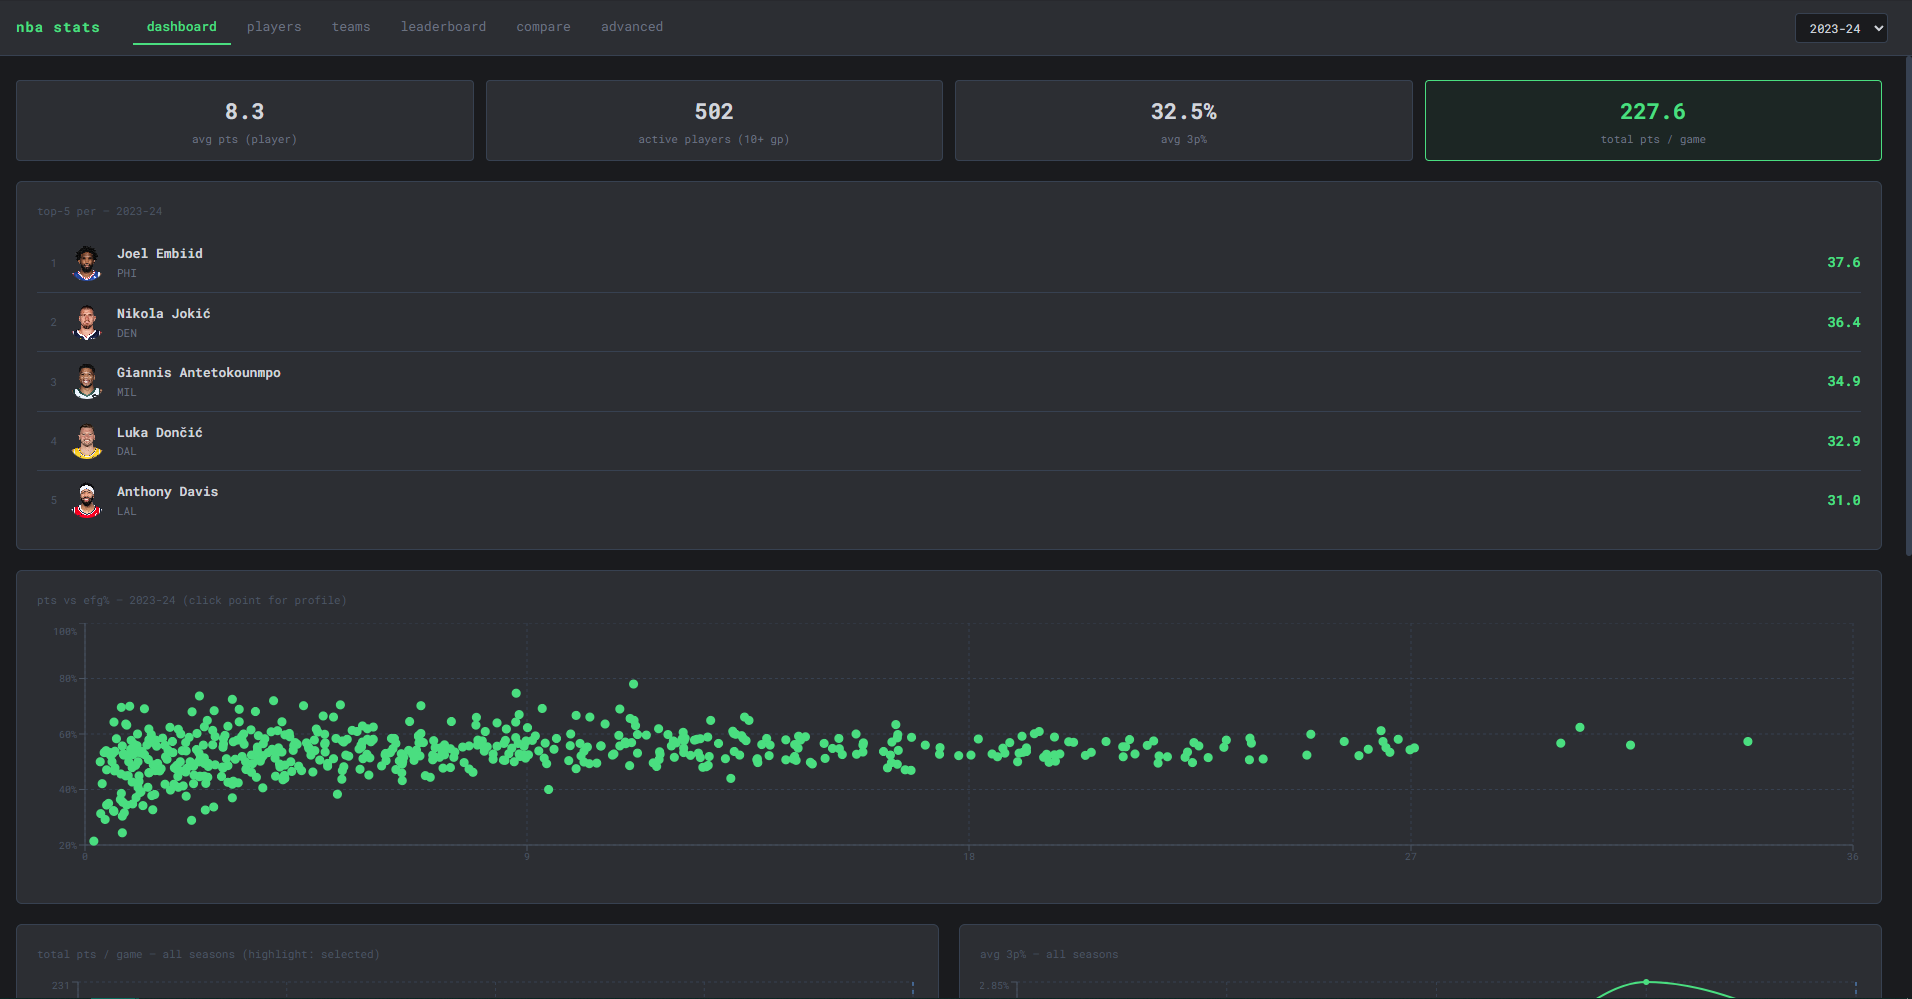
\includegraphics[width=\textwidth]{../img/dash.png}
\caption{Главная страница приложения (Dashboard)}
\label{fig:ui-dashboard}
\end{figure}

\begin{figure}[H]
\centering
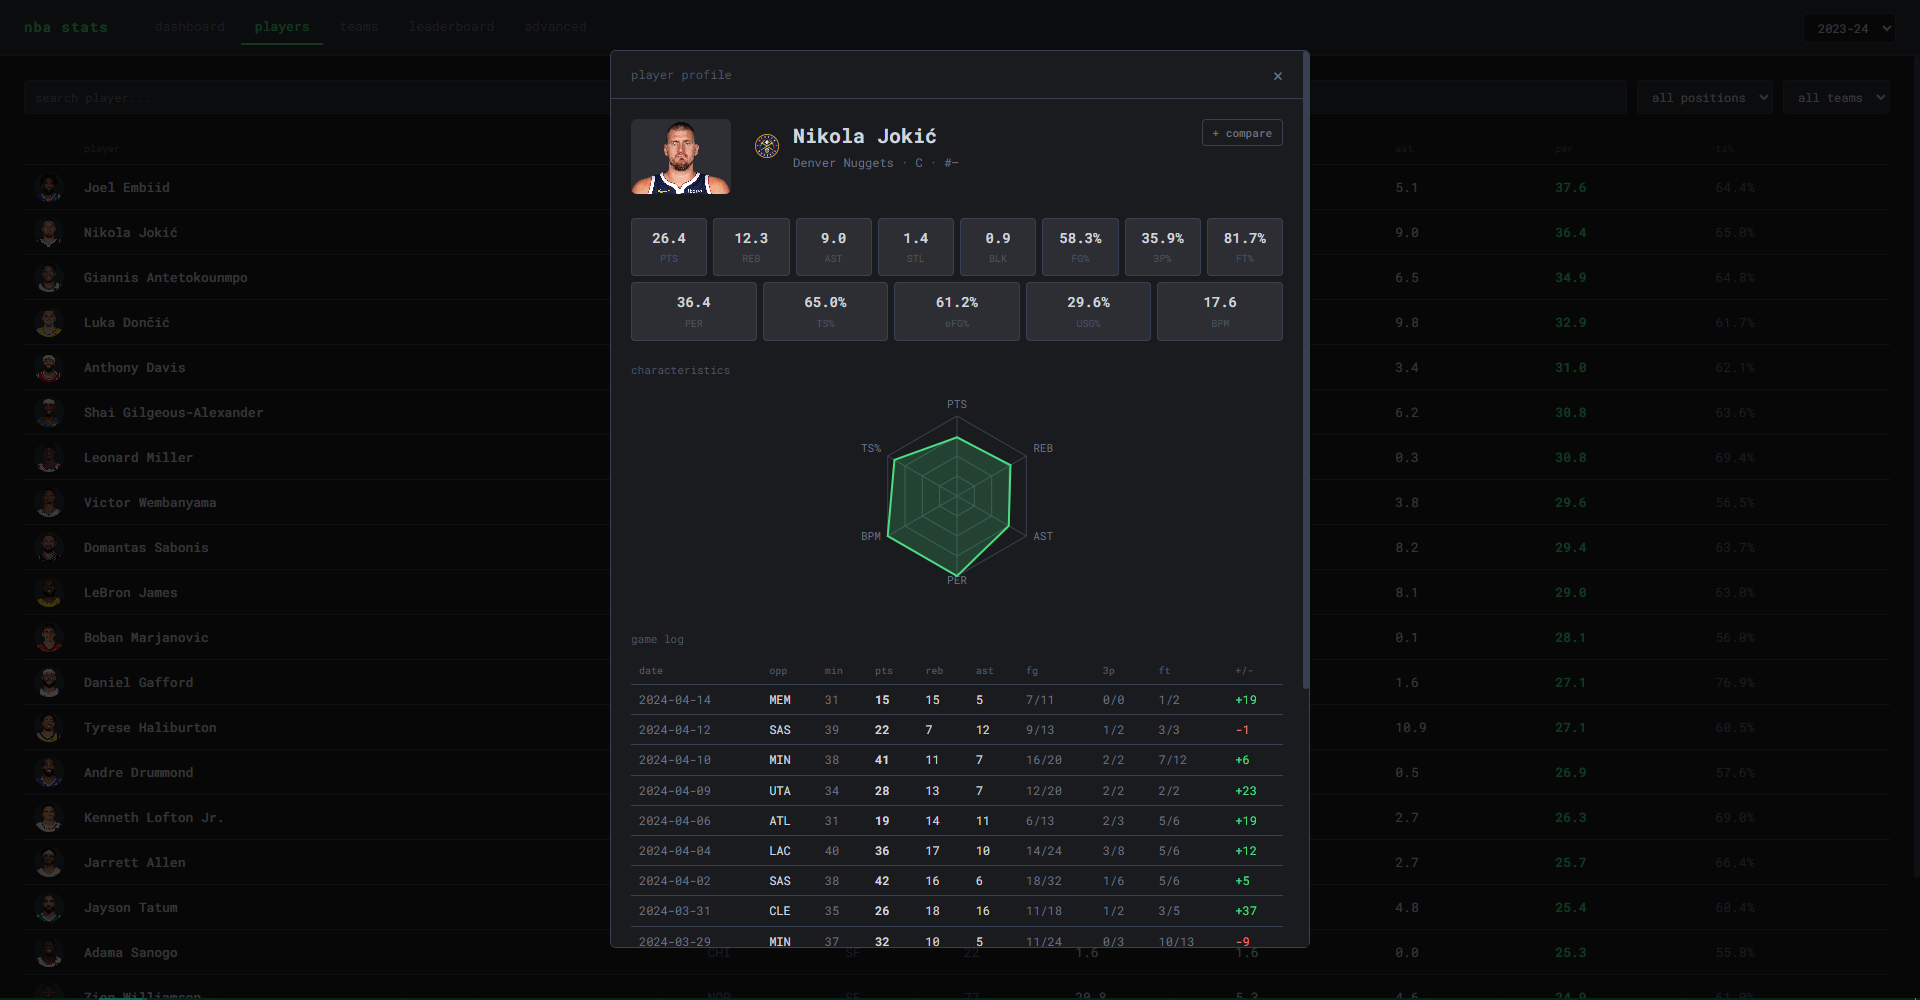
\includegraphics[width=\textwidth]{../img/player.png}
\caption{Модальное окно профиля игрока: сезонные метрики и игровой журнал}
\label{fig:ui-modal}
\end{figure}

\begin{figure}[H]
\centering
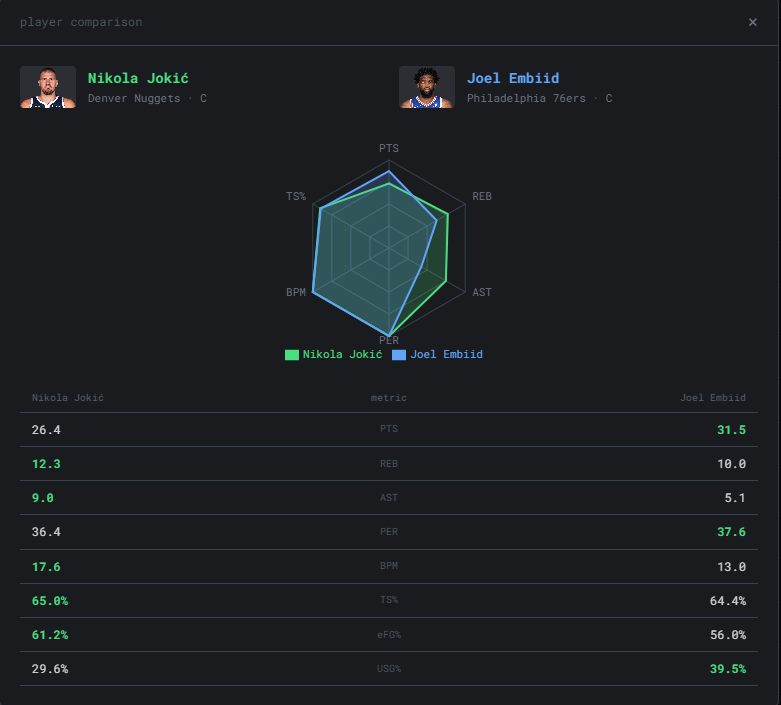
\includegraphics[width=0.8\textwidth]{../img/comp.png}
\caption{Модальное окно сравнения профилей двух игроков}
\label{fig:ui-compare}
\end{figure}


\section*{Приложение Е. Презентация}
\addcontentsline{toc}{section}{Приложение Е. Презентация}

\noindent презентация

